\documentclass[20pt]{article}
\usepackage{fullpage}
\usepackage{graphicx}
\usepackage{color}
\usepackage[utf8]{inputenc}
\usepackage[spanish]{babel}

\begin{document}

\begin{center}
\begin{huge}
\textbf{Cinema}\\\
\end{huge}
\end{center}

\begin{center}
\begin{huge}
\textbf{Manual de usuario}\\\
\end{huge}
\end{center}


\begin{large}
\textbf{1:Inicio de sesión}\\\
\end{large}

\begin{figure}[h]
\begin{center}
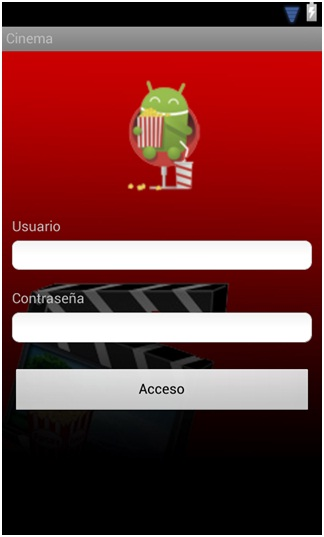
\includegraphics[width=100 pt]{./inicio.jpg}
\end{center}
\end{figure}

Al iniciar la aplicación se presentara esta pantalla que representa el inicio de sesión. En el primer cuadro de texto se ingresa el usuario registrado en el cine. En el segundo cuadro se ingresa la contraseña, que es el numero de cedula perteneciente al usuario. Una vez ingresados ambos campos se podrá acceder al sistema.\\\\\



\begin{large}
\textbf{2:Menu principal}\\\
\end{large}

\begin{figure}[h]
\begin{center}
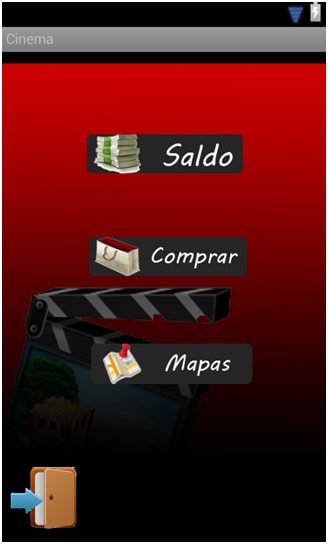
\includegraphics[width=100 pt]{./menu_principal.jpg}
\end{center}
\end{figure}

En el menú principal se mostraran cuatro opciones: 

\begin{itemize}
\item Saldo: aquí se muestra el saldo disponible en la cuenta.
\item Comprar: se catalogan las ventas que ofrece el cine para el usuario.
\item Mapas: se muestran las ubicaciones geográficas de los distintos locales del cine dentro de la ciudad.
\item Cerrar sesión.
\end{itemize}



\begin{large}
\textbf{3:Saldo disponible}\\\
\end{large}

\begin{figure}[h]
\begin{center}
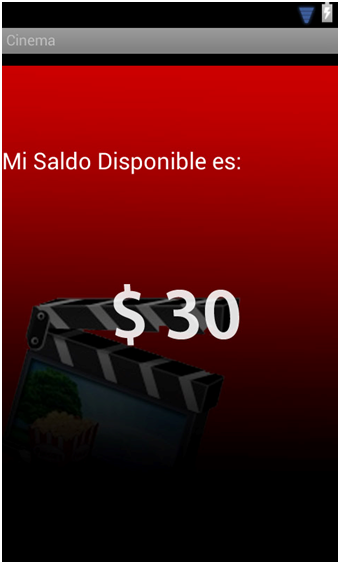
\includegraphics[width=100 pt]{./saldo_disponible.jpg}
\end{center}
\end{figure}

Se muestra el saldo disponible en la cuenta del usuario.
Para regresar al menú principal, se presiona el botón “deshacer” del Smartphone.\\\\\\

\begin{large}
\textbf{4:Comprar}\\\
\end{large}


\begin{enumerate}
\item Seleccion de cine\\Al seleccionar en el menú principal “Comprar”, el usuario debe de seleccionar en que cine se encuentra para seguir con el debido procedimiento de la compra.
\begin{figure}[h]
\begin{center}
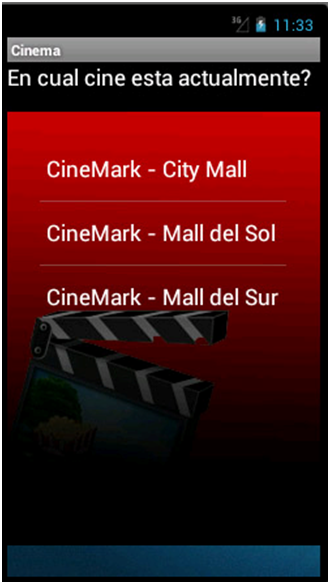
\includegraphics[width=100 pt]{./seleccion_de_cine.jpg}
\end{center}
\end{figure}

\item Datos de factura\\
Se ingresa el código de la factura que viene impreso en el ticket, como se indica en la figura.
Mediante este código se obtiene la función, el asiento, la sala y los datos personales del usuario necesarios para que el cine facture la compra.

\begin{figure}[h]
\begin{center}
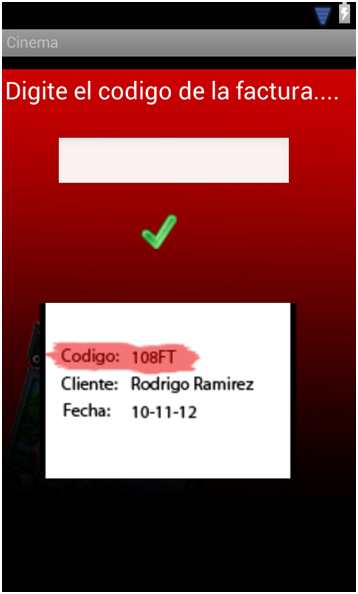
\includegraphics[width=100 pt]{./datos_de_factura.jpg}
\end{center}
\end{figure}

\item Menu de compra\\
\begin{figure}[h]
\begin{center}
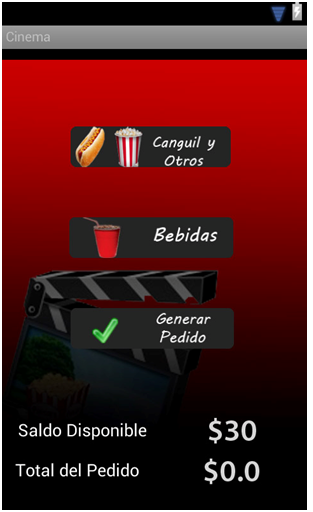
\includegraphics[width=100 pt]{./menu_de_compra.jpg}
\end{center}
\end{figure}
En el menú principal se mostraran dos opciones: 
\begin{itemize}
\item Canguil y otros: se muestran los snacks. 
\item Bebidas: se muestran las bebidas con sus tamaños.
\end{itemize}

Una vez que se seleccionan las compras, se oprime generar pedido y se genera la factura. Adicionalmente se muestran el saldo disponible en cada momento y el total del pedido.

\item Canguil y otros
Se muestran los distintos snacks que ofrece el cine. Se debe seleccionar solo uno por compra. Para hacer esto, se presiona uno de los iconos mostrados y luego se oprime el visto verde para aceptar la compra.

\begin{figure}[h]
\begin{center}
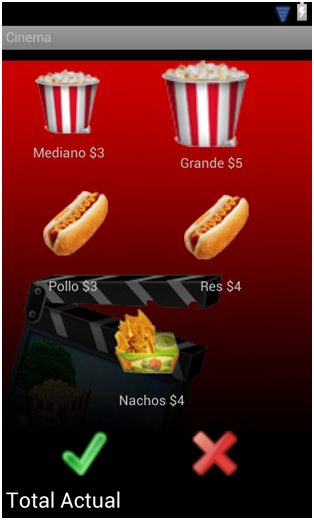
\includegraphics[width=100 pt]{./canguil_y_otros.jpg}
\end{center}
\end{figure}


\end{enumerate}





\end{document}